\documentclass[10pt]{article}
\usepackage{geometry}                % See geometry.pdf to learn the layout options. There are lots.
\geometry{a4paper
}                   % ... or a4paper or a5paper or ... 
\usepackage[parfill]{parskip}    % Activate to begin paragraphs with an empty line rather than an indent

%%%%%%%%%%%%%%%%%%%%
\newcommand{\hide}[1]{}

\usepackage{natbib}
\usepackage{xcolor}
\usepackage{url}
\usepackage{hyperref}
\usepackage{mathtools}
\usepackage{array}
\usepackage{multirow}
\usepackage{graphicx}
\usepackage{subcaption}
\usepackage{mwe}
\usepackage{float}
\usepackage{tikz}

\hide{
\usepackage{amscd}
\usepackage{amsfonts}
\usepackage{amsmath}
\usepackage{amssymb}
\usepackage{amsthm}
\usepackage{cases}		 
\usepackage{cutwin}
\usepackage{enumerate}
\usepackage{epstopdf}
\usepackage{graphicx}
\usepackage{ifthen}
\usepackage{lipsum}
\usepackage{mathrsfs}	
\usepackage{multimedia}
\usepackage{wrapfig}
}

	 
%\input{/usr/local/LATEX/Lee_newcommands.tex}
\newcommand{\itemlist}[1]{\begin{itemize}#1\end{itemize}}
\newcommand{\enumlist}[1]{\begin{enumerate}#1\end{enumerate}}
\newcommand{\desclist}[1]{\begin{description}#1\end{description}}

\newcommand{\Answer}[1]{\begin{quote}{\color{blue}#1}\end{quote}}
\newcommand{\AND}{\wedge}
\newcommand{\OR}{\vee}
\newcommand{\ra}{\rightarrow}
\newcommand{\lra}{\leftrightarrow}

\title {CS36110 Machine Learning Assignment}


\date{}                                           % Activate to display a given date or no date

\begin{document}
\maketitle

\section*{Task 1}

\subsection*{Part A}
The first algorithm I used was the C4.5 Decision Tree classifier this is an implementation of the ID3 algorithm with Rule Post-Pruning. ID3 grows a decision tree recursively where at each node it selects the feature with the highest information gain that best classifies the training data it was given, when the tree is grown Rule Post-Pruning (RPP) is then run over the entire tree. RPP converts each path through the tree to a rule and then independently evaluates each rule to see if it affects the validation accuracy of the tree and if it doesn't then it is pruned out. C4.5 mitigates overfiting because it uses RPP this helps the algorithm make a decision tree that more accurately fits the patterns in the data instead of fitting to the data itself.

The second classifier I used was Naive Bayes and it works by calculating the probabilities of events occurring within the data set it does this using Bayes Theorem which is shown in Figure \ref{fig:bayes} and works be relating the Posterior Probability $(P(A \mid B))$ with the prior probability of the hypothesis $(P(A))$ and the conditional probability of the data under the hypothesis $(P(B \mid A))$. To classify a new piece of data you work out the probability for each decision class using the training data and the class with the highest probability is the one that you assign that data to. Naive Bayes doesn't go through a long training sequence so this makes it very fast when you want to classify a piece of data, this also makes it quick and easy to update when you get new training data.

An advantage C4.5 has over Naive Bayes is that Naive Bayes assumes that all the data is independent which isn't true in real life applications this can result in a poor accuracy of the trained model.


\begin{figure}[h]
    \centering
    $$ P(A \mid B) = \frac{P(B \mid A) \, P(A)}{P(B)} $$
    \caption{Bayes Theorem}
    \label{fig:bayes}
\end{figure}

\newpage
\subsection*{Part B}
Over the entire training data set the C4.5 model obtained a recall measurement of 71.9\% compared to Naive Bayes 55.7\%, recall is a measure of of the ratio of the number of correct positive examples out of those which were classified as positive\cite{MarslandStephen2015Ml:a} a higher recall measure means that more instances are being correctly classified. Precision is the ratio of correct positive examples to the number of actual positive examples\cite{MarslandStephen2015Ml:a}, the precision for C4.5 is 71.8\% and for Naive Bayes it is 58.7\% the higher precision means that the classifier successfully classified more results. 

A useful measure for evaluating classifiers is the Receiver Operator Characteristic Curve this is a plot of false positive rate along the x axis and true positive rate along the y axis, a perfect classifier would be a plot at (0,1) which would mean 100\% true positives and 0\% false positives. Figures \ref{fig:naive bayes roc curves} and \ref{fig:c45 roc curves} show these ROC curves and says their Area Under Curve (AUC), these two figures show you how much better the C4.5 classifier is when compared to Naive Bayes. The AUC represents how good the classifier is at distinguishing between classes, on average the AUC for the C4.5 classes is higher than for Naive Bayes so C4.5 is better at classifying the absences. 


\begin{figure*}[h]
    \centering
    \begin{subfigure}[b]{0.475\textwidth}
        \centering
        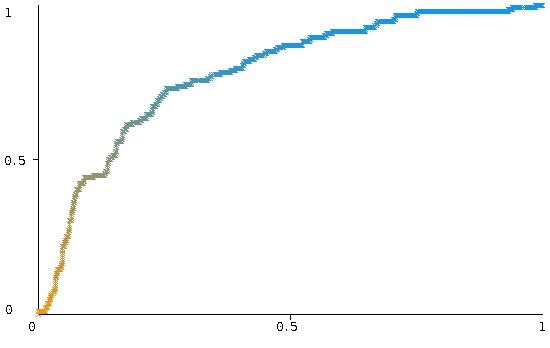
\includegraphics[width=\textwidth]{bayes_roc/roc_curve_a.jpg}
        \caption[Network2]%
        {{\small The ROC for class a, the area under ROC is 0.7803}}    
        \label{fig:bayes roc curve class a}
    \end{subfigure}
    \hfill
    \begin{subfigure}[b]{0.475\textwidth}  
        \centering 
        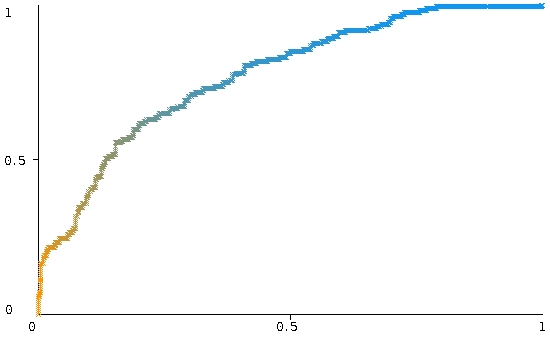
\includegraphics[width=\textwidth]{bayes_roc/roc_curve_b.jpg}
        \caption[]%
        {{\small The ROC for class b, the area under ROC is 0.7723}}    
        \label{fig:bayes roc curve class b}
    \end{subfigure}
    \vskip\baselineskip
    \begin{subfigure}[b]{0.475\textwidth}   
        \centering 
        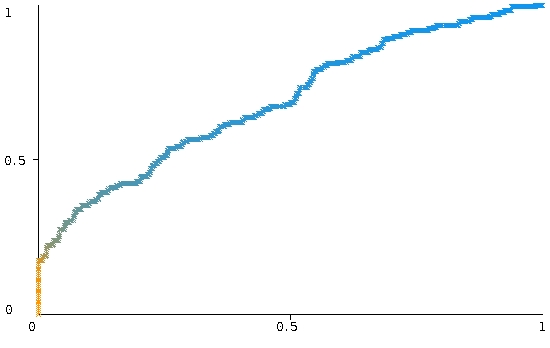
\includegraphics[width=\textwidth]{bayes_roc/roc_curve_c.jpg}
        \caption[]%
        {{\small The ROC for class c, the area under ROC is 0.6881}}    
        \label{fig:bayes roc curve class c}
    \end{subfigure}
    \quad
    \begin{subfigure}[b]{0.475\textwidth}   
        \centering 
        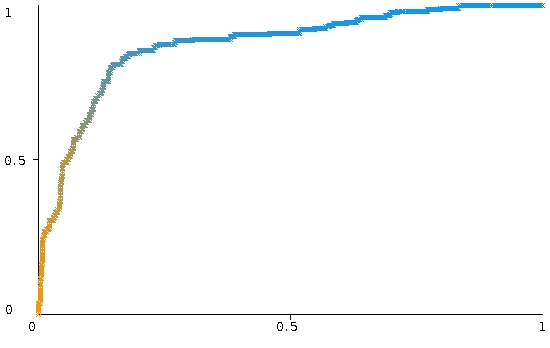
\includegraphics[width=\textwidth]{bayes_roc/roc_curve_e(d).jpg}
        \caption[]%
        {{\small The ROC for class d, the area under ROC is 0.8715}}    
        \label{fig:bayes roc curve class d}
    \end{subfigure}
    \caption[ ]
    {\small The Receiver Operator Characteristic Curve for the Naive Bayes classifier} 
    \label{fig:naive bayes roc curves}
\end{figure*}

\begin{figure*}[ht]
    \centering
    \begin{subfigure}[b]{0.475\textwidth}
        \centering
        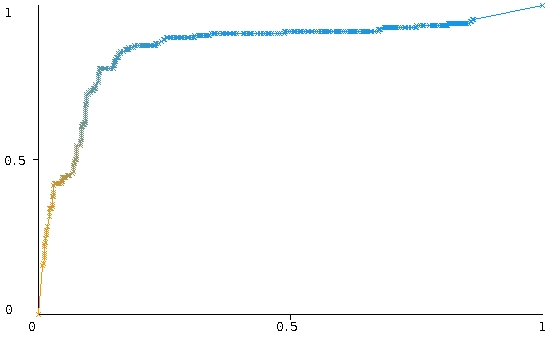
\includegraphics[width=\textwidth]{c45_roc/roc_curve_a.jpg}
        \caption[Network2]%
        {{\small The ROC for class a, the area under ROC is 0.8613}}    
        \label{fig:c45 roc curve class a}
    \end{subfigure}
    \hfill
    \begin{subfigure}[b]{0.475\textwidth}  
        \centering 
        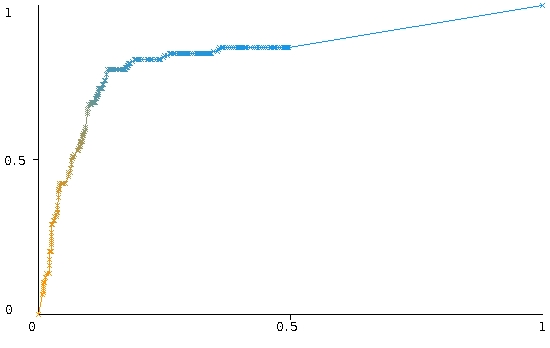
\includegraphics[width=\textwidth]{c45_roc/roc_curve_b.jpg}
        \caption[]%
        {{\small The ROC for class b, the area under ROC is 0.8341}}    
        \label{fig:c45 roc curve class b}
    \end{subfigure}
    \vskip\baselineskip
    \begin{subfigure}[b]{0.475\textwidth}   
        \centering 
        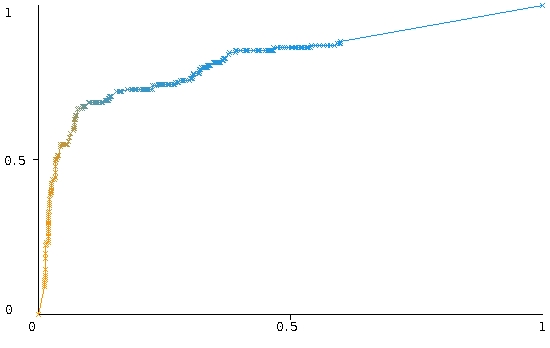
\includegraphics[width=\textwidth]{c45_roc/roc_curve_c.jpg}
        \caption[]%
        {{\small The ROC for class c, the area under ROC is 0.8208}}    
        \label{fig:c45 roc curve class c}
    \end{subfigure}
    \quad
    \begin{subfigure}[b]{0.475\textwidth}   
        \centering 
        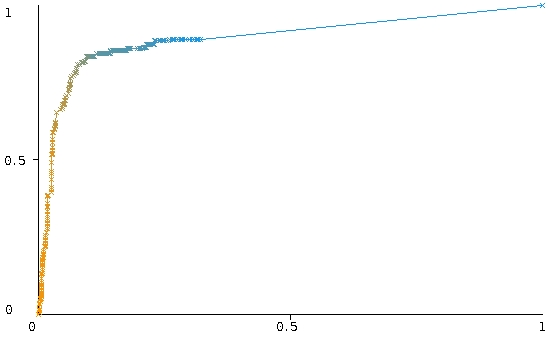
\includegraphics[width=\textwidth]{c45_roc/roc_curve_e(d).jpg}
        \caption[]%
        {{\small The ROC for class d, the area under ROC is 0.892}}    
        \label{fig:c45 roc curve class d}
    \end{subfigure}
    \caption[ ]
    {\small The Receiver Operator Characteristic Curve for the C4.5 Classifier} 
    \label{fig:c45 roc curves}
\end{figure*}



\subsection*{Part C}
Randomness is a good baseline to test against, a classifier that randomly chooses one of the four absence classes. If you used this over a dataset that had an equal number of instances from each class then you would expect an accuracy of around 25\%. This would be a good baseline because it's very easy to implement and very fast to do. 

\section*{Task 2}

\subsection*{Part A}
There are a few missing values in the Reason\_for\_absence and the Month\_of\_absence features, there are a few different ways of handling missing values. You could remove the missing values entirely so that data is no longer in the set   

\section*{Task 3}


\bibliographystyle{plain}
\nocite{*}
\bibliography{bibliography.bib}


\end{document}  
%%%%%%%%%%%%%%%%%%%%%%%%%%%%%%%%%%%%%%%%%%%%%%